\subsection{Procedure of template fitting}
\begin{frame}{Template fitting to evaluate background}
  \centering
  $d(K^, n \pi^- \pi^+)"n"$ event.
  \begin{tabular}{ccc}
    \begin{minipage}{0.33\hsize}
      \centering
      $\pi^+ \pi^-$ IM\\
      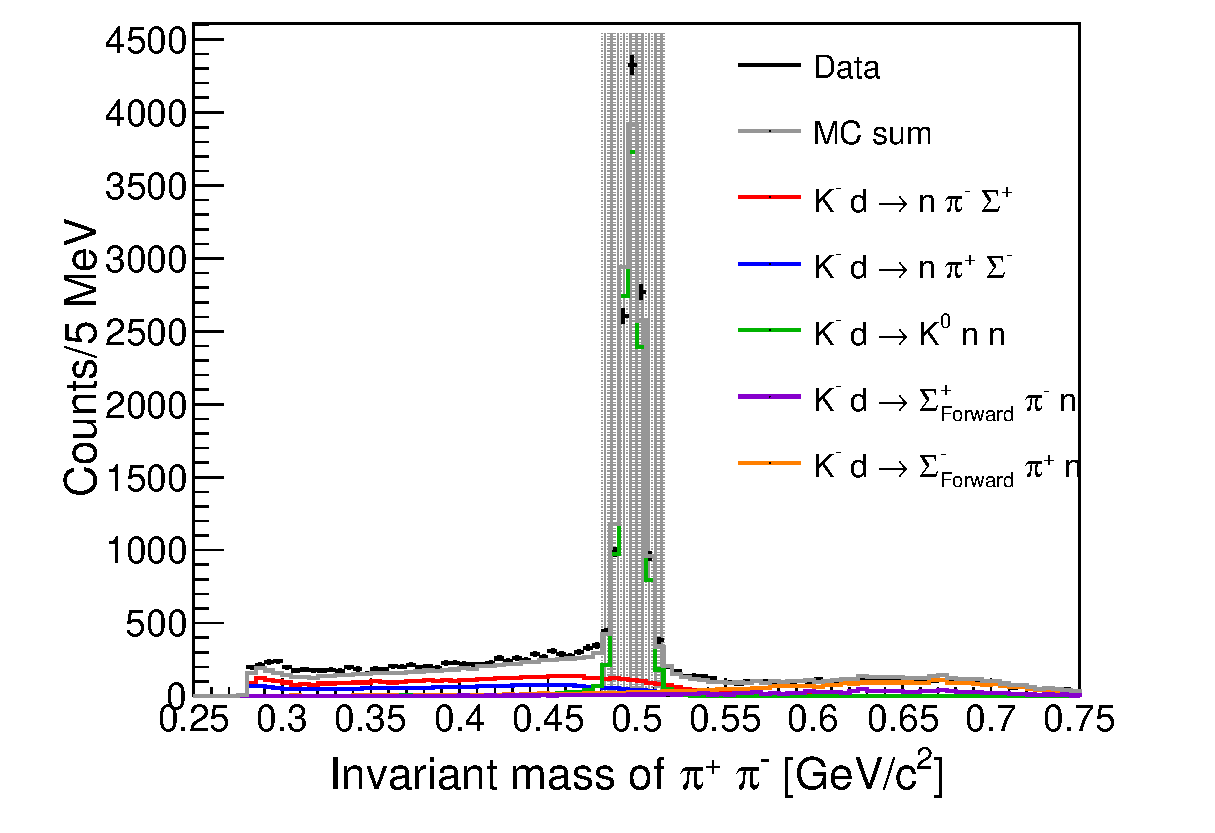
\includegraphics[width=4cm]{../pic/Dron/KN_ana/IM_pipi.eps}
    \end{minipage}
    \begin{minipage}{0.33\hsize}
      \centering
      $n_{forward} \pi^+$ IM\\
      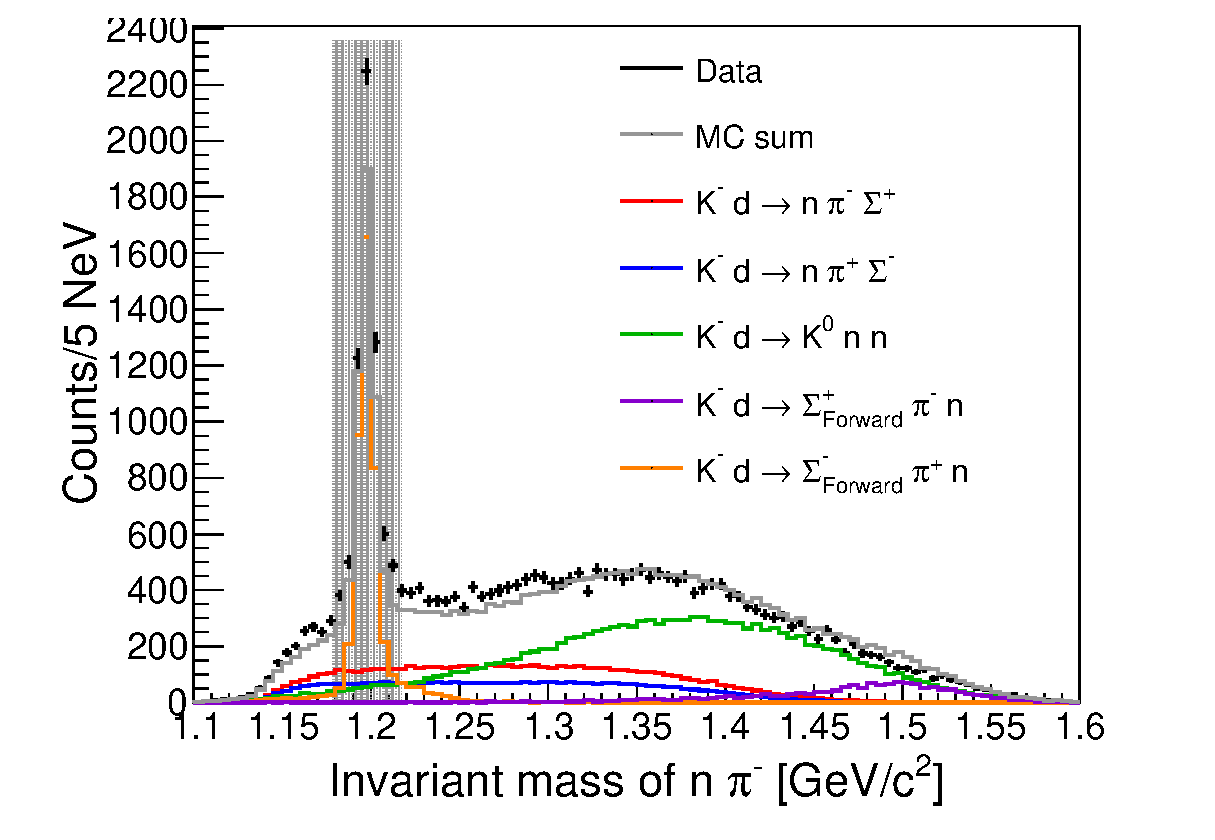
\includegraphics[width=4cm]{../pic/Dron/KN_ana/IM_npim.eps}
    \end{minipage}
    \begin{minipage}{0.33\hsize}
      \centering
      $n_{forward} \pi^-$ IM\\
      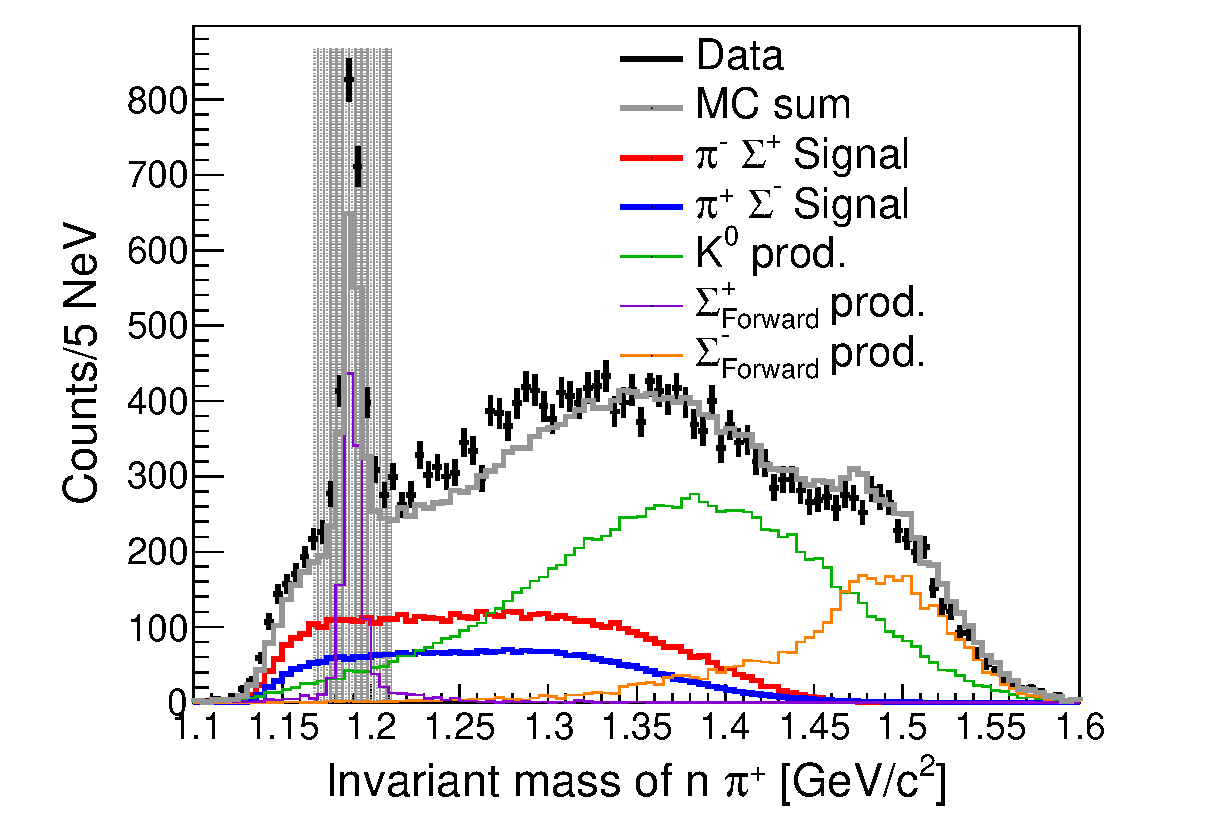
\includegraphics[width=4cm]{../pic/Dron/KN_ana/IM_npip.eps}
    \end{minipage}
  \end{tabular}
  \vspace{4mm}\\
  Each spectra are well reproduced. 
\end{frame}

\begin{figure}[htbp]
  \centering
  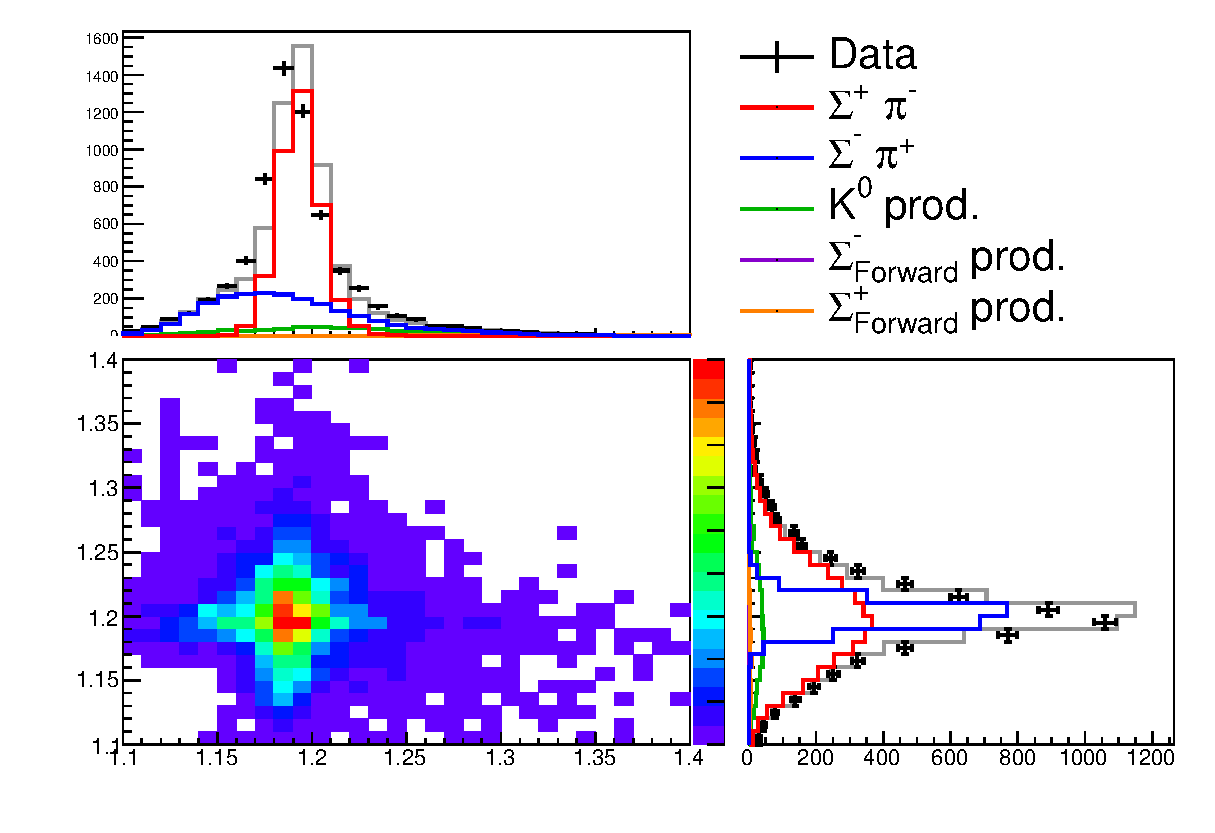
\includegraphics[width=12cm]{../pic/Run78/KN_ana_NC170_2sigma/KNpim_KNpip_MM.eps}
  \caption{
    This figure shows template fitting of the $d(K^-, n \pi)$ spectra to separate the $\pi^-\Sigma^+$ and $\pi^+ \Sigma^-$ modes.
    The lower left figure shows two-dimensional plots of $d(K^-, n \pi^-)$ and $d(K^-, n \pi^+)$ on the horizontal and vertical axes, respectively.
    The top and right panels show the projections onto each axis.
    The caption is the same as that of Figure.\ref{fig:fit_IM}.
  }
  \label{fig:fit_KNpi_MM_all}
\end{figure}


In this subsection, we explain procedure of template fitting, whose main purpose is decomposition of $\pi^- \Sigma^+$ and $\pi^+ \Sigma^-$ modes.
Template fitting is divided into two stages, one fitting to estimate the amount of background for $K^0$ and $\Sigma_{forward}$ production,
the other to separate $\pi^-\Sigma^+$ and $\pi^+\Sigma^-$ modes.
These fittings are performed using fitting with the likelihood method on a finite sample generated by Monte Carlo method\cite{temp_fit}.
There is no $\chi^2$ in this fitting,
but there is a value of $-2\log\Lambda$ that asymptotically approaches the $\chi^2$ when the number of samples become infinite, and the fitting is evaluated with this value.
Here, $\Lambda$ is the likelihood.

The first fitting is performed using the invariant mass distributions of $\pi^+ \pi^-$, $n \pi^+$ and $n \pi^-$ in the event that $K^-d \rightarrow n \pi^+ \pi^- n$ final state.
The $K^0$, $\Sigma^+$ and $\Sigma^-$ productions create peaks in the respective invariant mass distributions as shown in Fig.\ref{fig:fit_IM}.
The distributions reconstructed by fitting are also plotted in the same figure.
The bold line represents the case of backward $\pi \Sigma$ production of signal, with red and blue representing the $\pi^- \Sigma^+$ and $\pi^-\Sigma^+$ modes, respectively.
The other green, purple and orange lines represent the background for $K^0$, $\Sigma^-_{forward}$ and $\Sigma^+_{forward}$ production, respectively.
This fitting of $-2\log\Lambda$ is \IMfitChiSquare.
Degrees freedom is the number of bin with data, and $-2\log\Lambda/NDF \sim $\IMfitChiNDF. 
% For this purpose, the distribution is fitted with a Gaussian and a 5-th polynomial function, and the rejection region is defined by the 3$\sigma$ of the Gaussian.

\begin{figure}
  \begin{tabular}{ccccc}
    \begin{minipage}{0.2\hsize}
      \includegraphics[width=2.2cm]{../pic/Run78/KN_ana_NC170_2sigma/KNpi_MM_0.eps}
    \end{minipage}
    \begin{minipage}{0.2\hsize}
      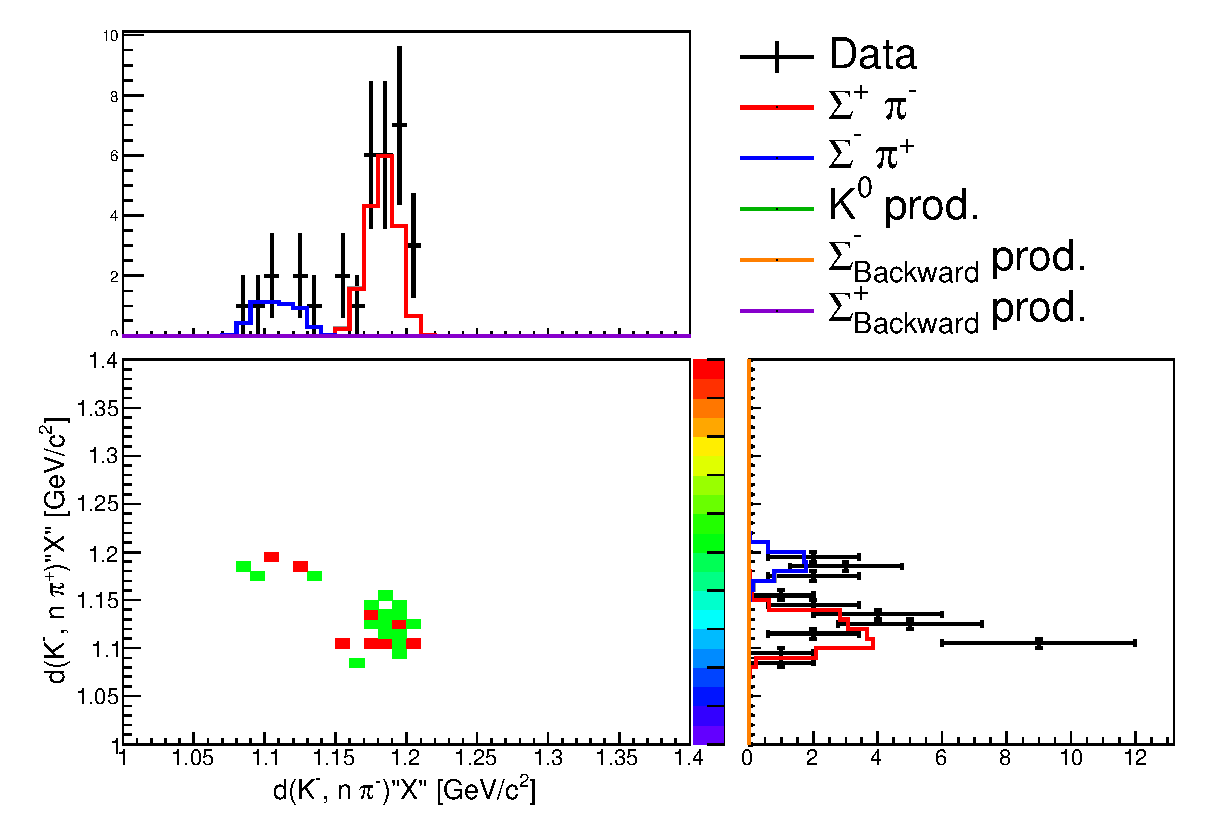
\includegraphics[width=2.2cm]{../pic/Run78/KN_ana_NC170_2sigma/KNpi_MM_1.eps}
    \end{minipage}
    \begin{minipage}{0.2\hsize}
      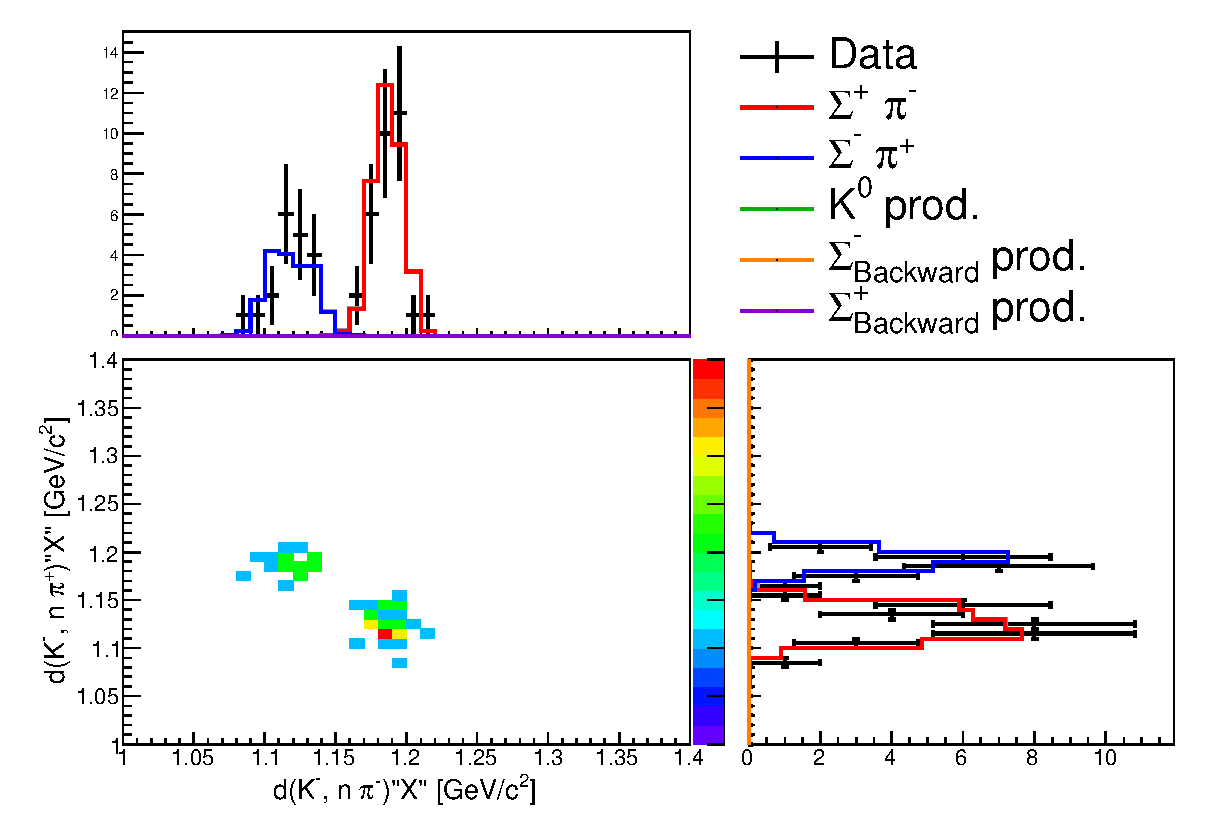
\includegraphics[width=2.2cm]{../pic/Run78/KN_ana_NC170_2sigma/KNpi_MM_2.eps}
    \end{minipage}
    \begin{minipage}{0.2\hsize}
      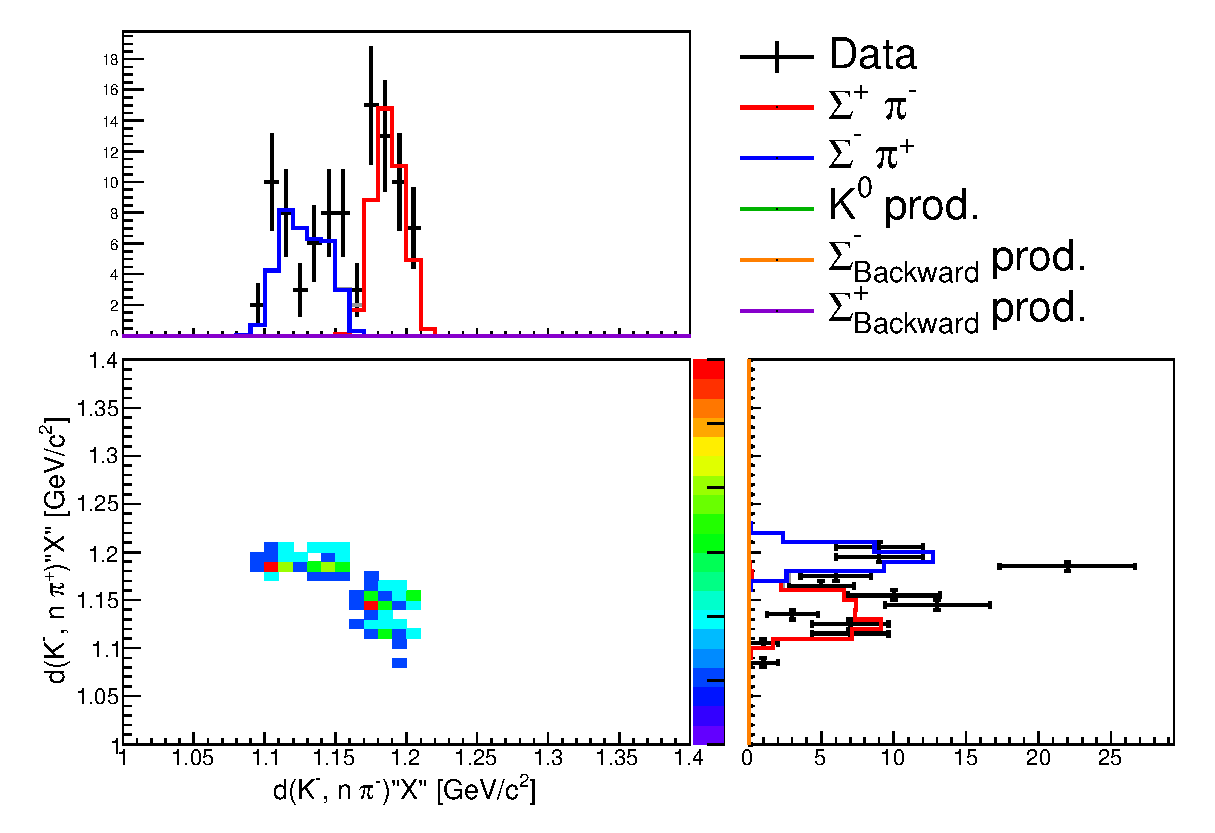
\includegraphics[width=2.2cm]{../pic/Run78/KN_ana_NC170_2sigma/KNpi_MM_3.eps}
    \end{minipage}
    \begin{minipage}{0.2\hsize}
      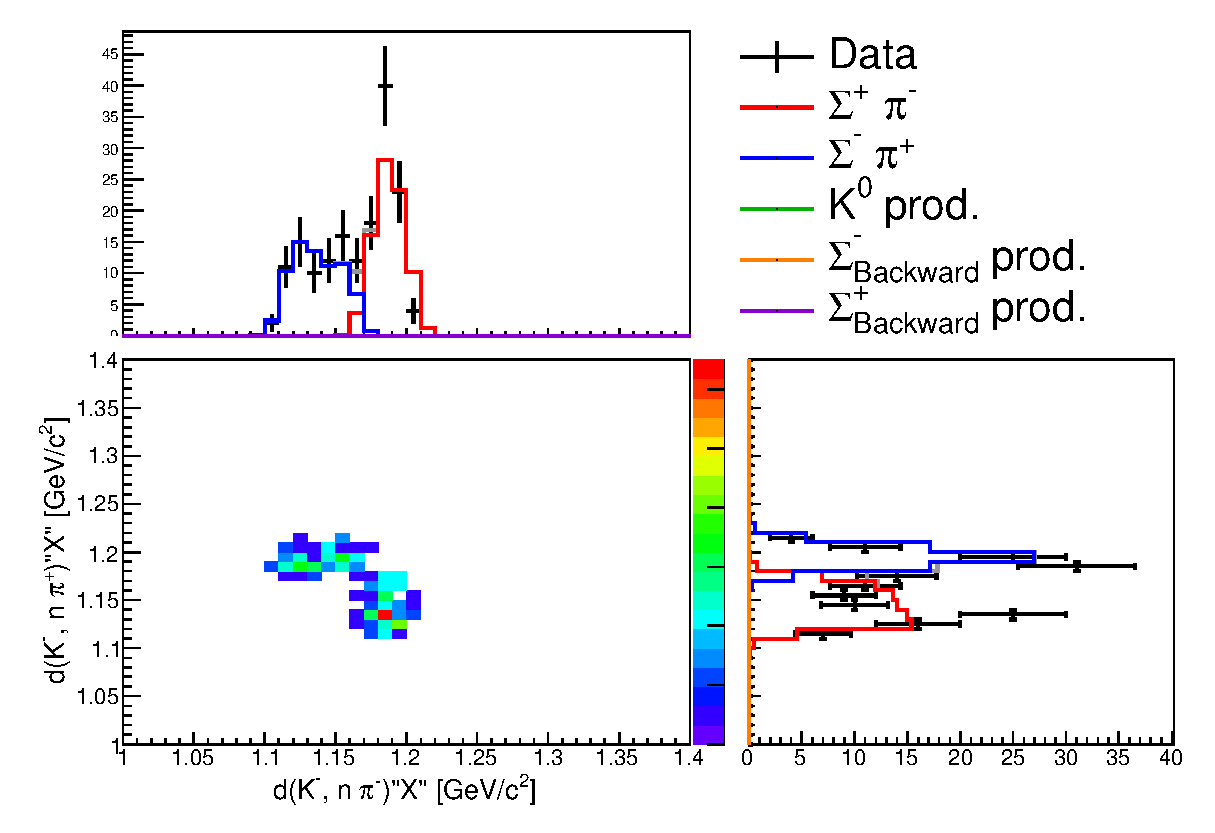
\includegraphics[width=2.2cm]{../pic/Run78/KN_ana_NC170_2sigma/KNpi_MM_4.eps}
    \end{minipage}
  \end{tabular}
  \begin{tabular}{ccccc}
    \begin{minipage}{0.2\hsize}
      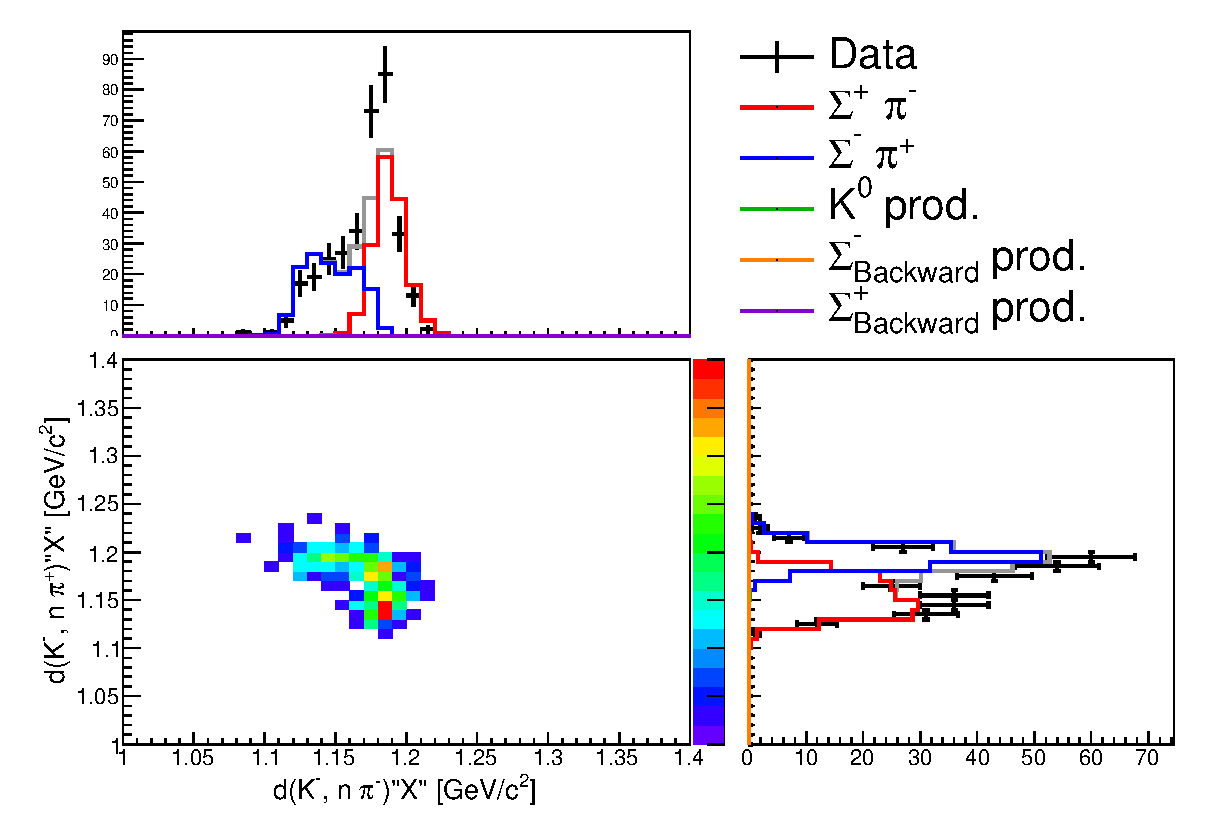
\includegraphics[width=2.2cm]{../pic/Run78/KN_ana_NC170_2sigma/KNpi_MM_5.eps}
    \end{minipage}
    \begin{minipage}{0.2\hsize}
      \includegraphics[width=2.2cm]{../pic/Run78/KN_ana_NC170_2sigma/KNpi_MM_6.eps}
    \end{minipage}
    \begin{minipage}{0.2\hsize}
      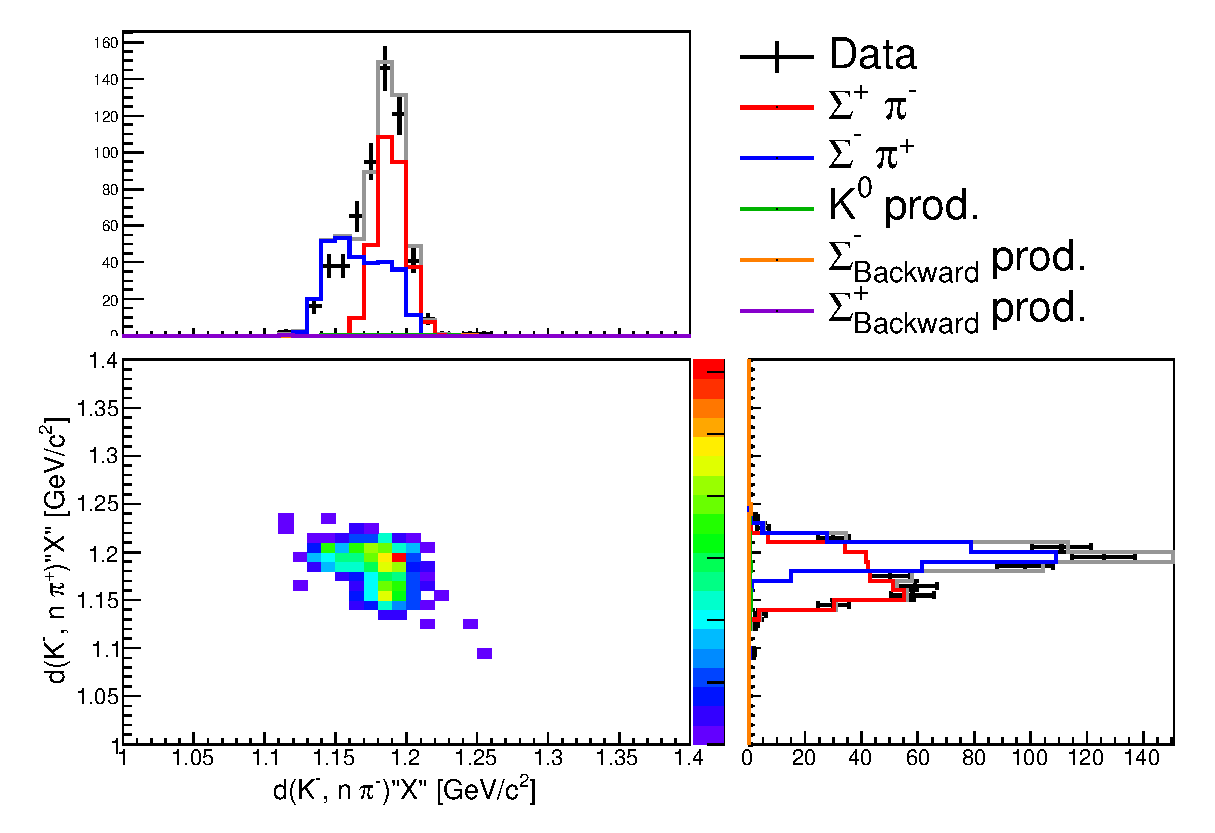
\includegraphics[width=2.2cm]{../pic/Run78/KN_ana_NC170_2sigma/KNpi_MM_7.eps}
    \end{minipage}
    \begin{minipage}{0.2\hsize}
      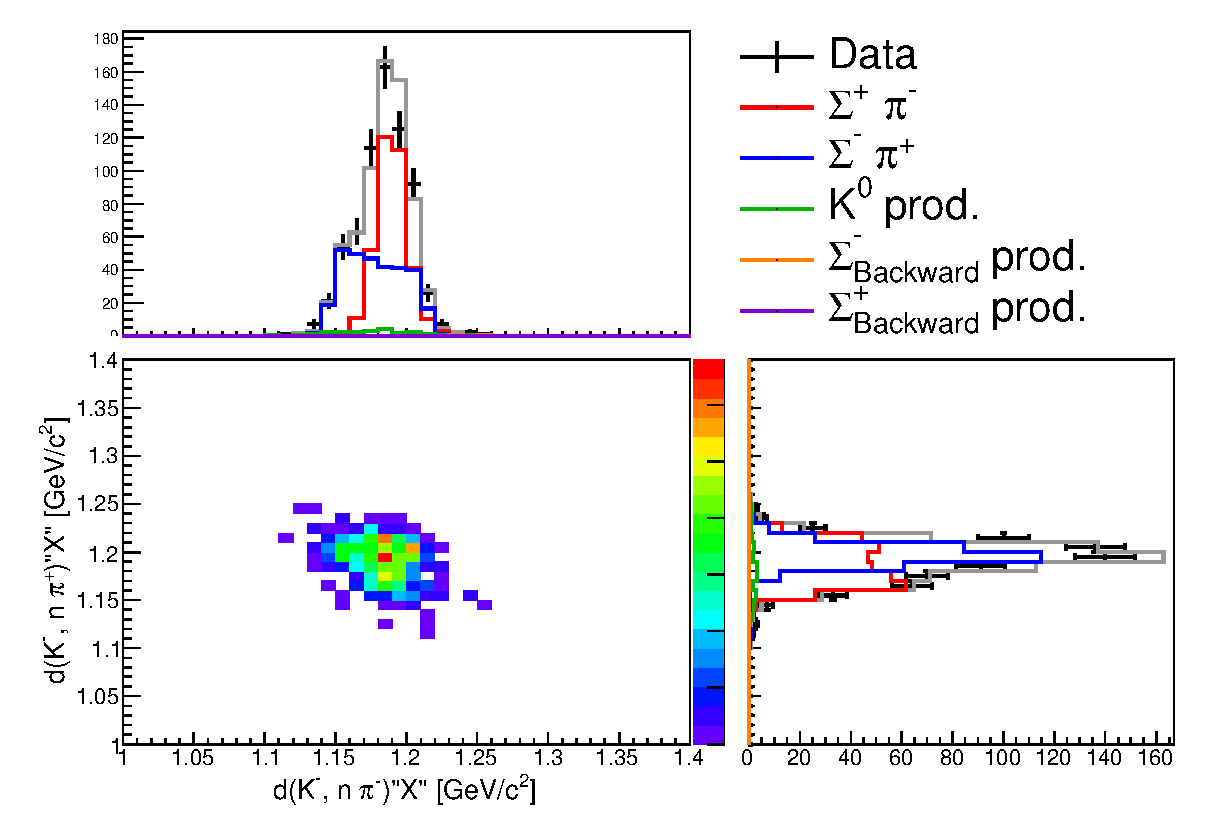
\includegraphics[width=2.2cm]{../pic/Run78/KN_ana_NC170_2sigma/KNpi_MM_8.eps}
    \end{minipage}
    \begin{minipage}{0.2\hsize}
      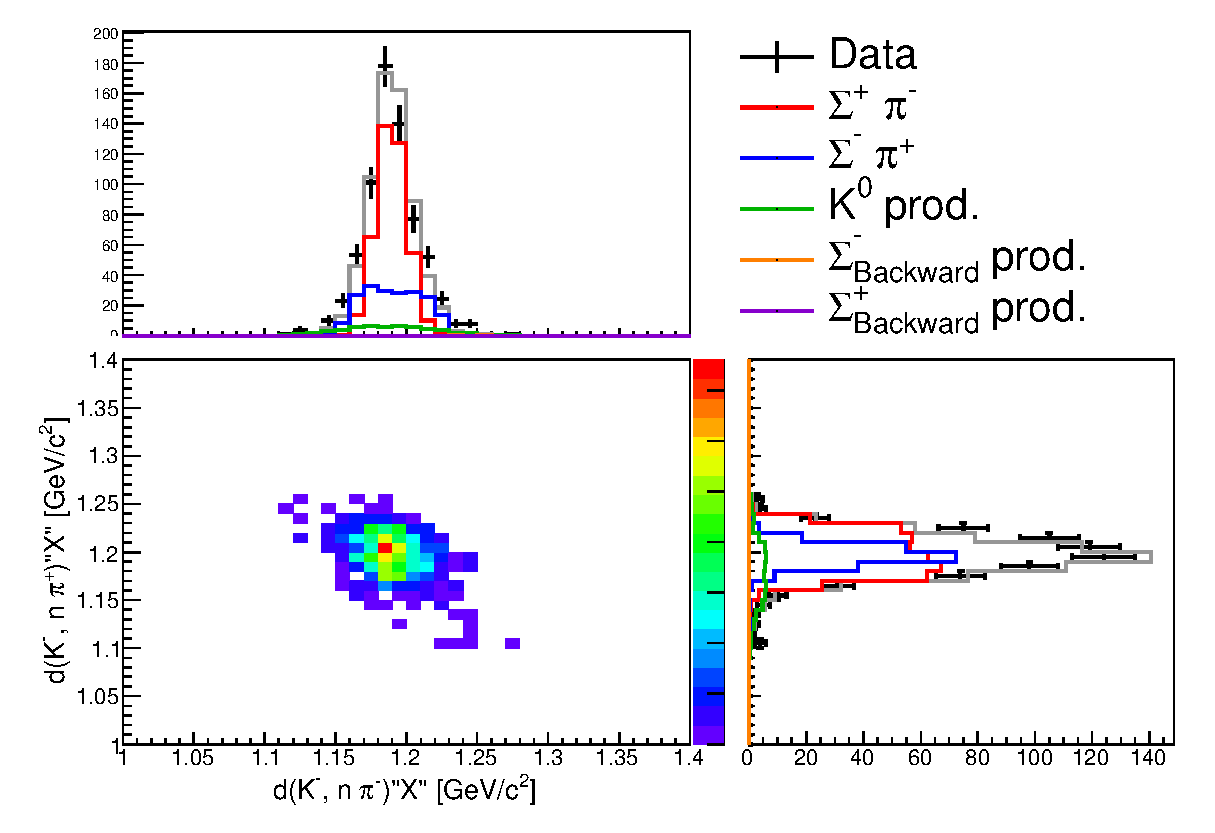
\includegraphics[width=2.2cm]{../pic/Run78/KN_ana_NC170_2sigma/KNpi_MM_9.eps}
    \end{minipage}
  \end{tabular}
  \begin{tabular}{ccccc}
    \begin{minipage}{0.2\hsize}
      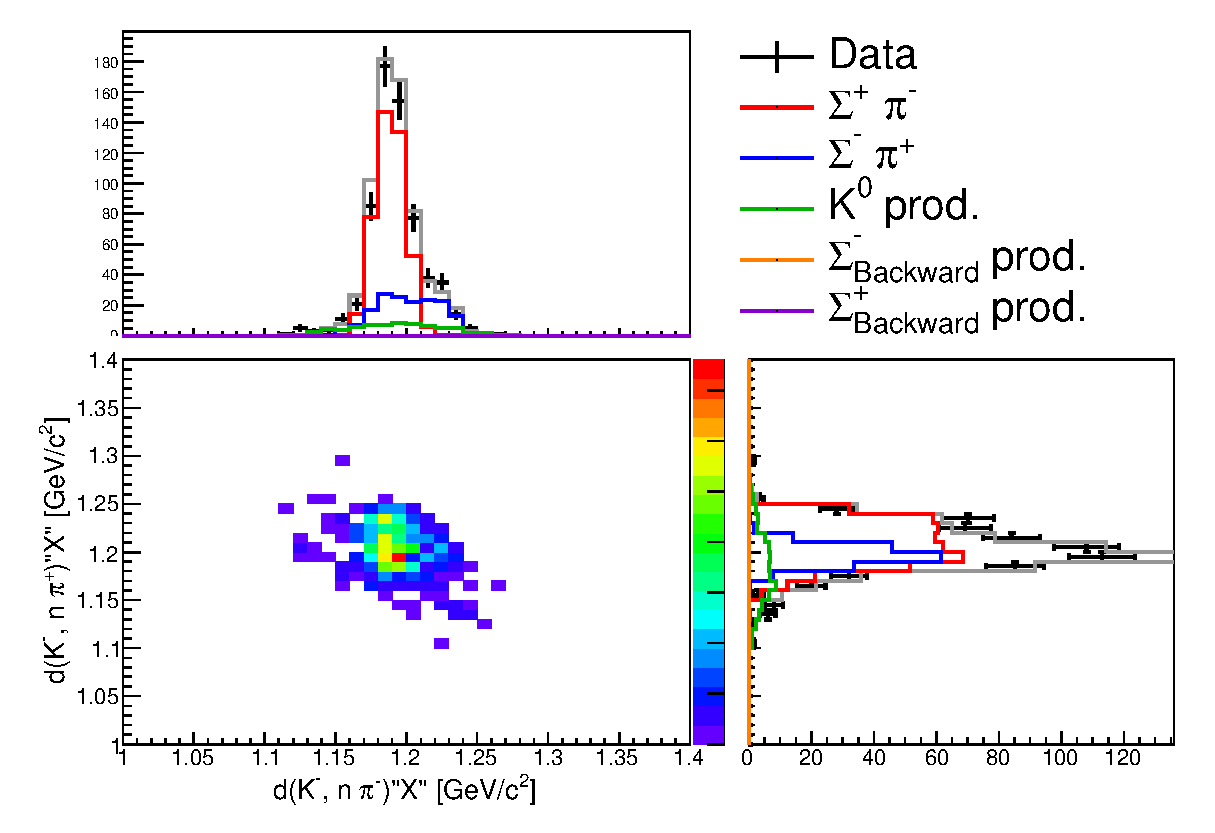
\includegraphics[width=2.2cm]{../pic/Run78/KN_ana_NC170_2sigma/KNpi_MM_10.eps}
    \end{minipage}
    \begin{minipage}{0.2\hsize}
      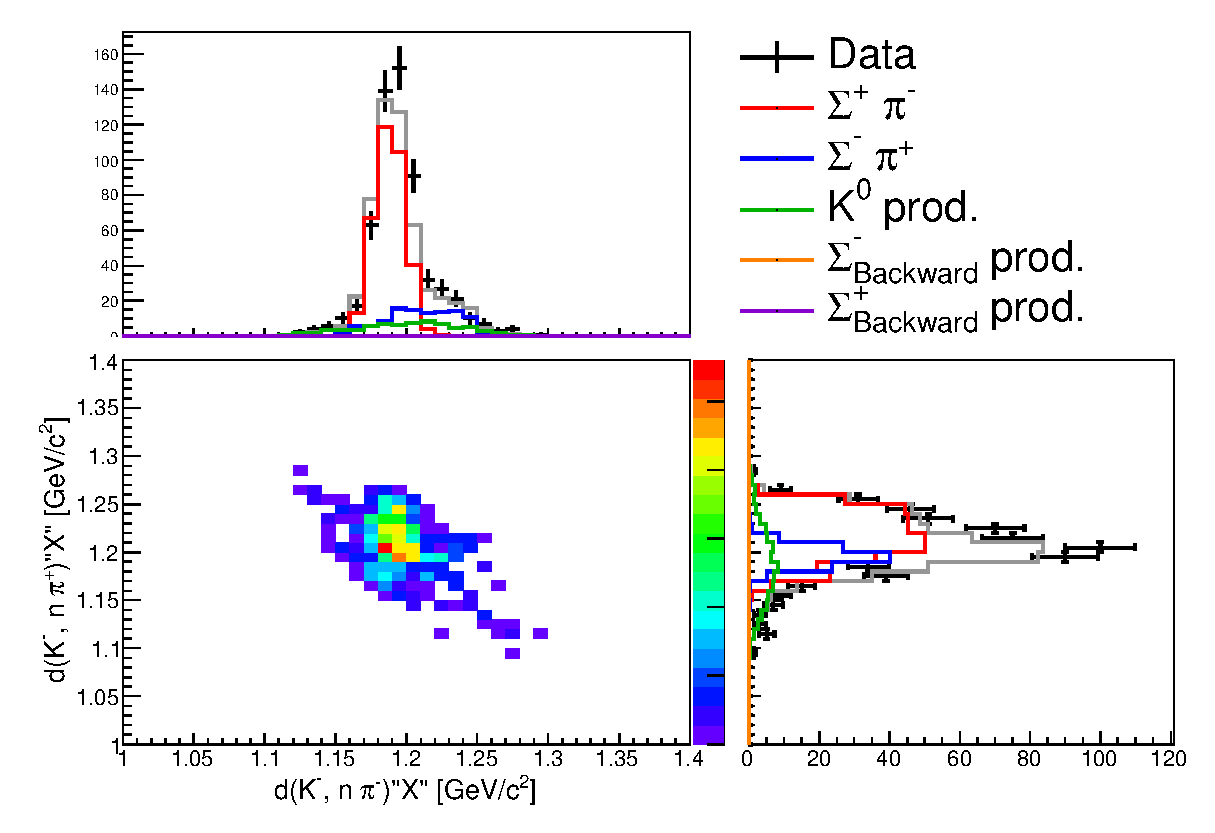
\includegraphics[width=2.2cm]{../pic/Run78/KN_ana_NC170_2sigma/KNpi_MM_11.eps}
    \end{minipage}
    \begin{minipage}{0.2\hsize}
      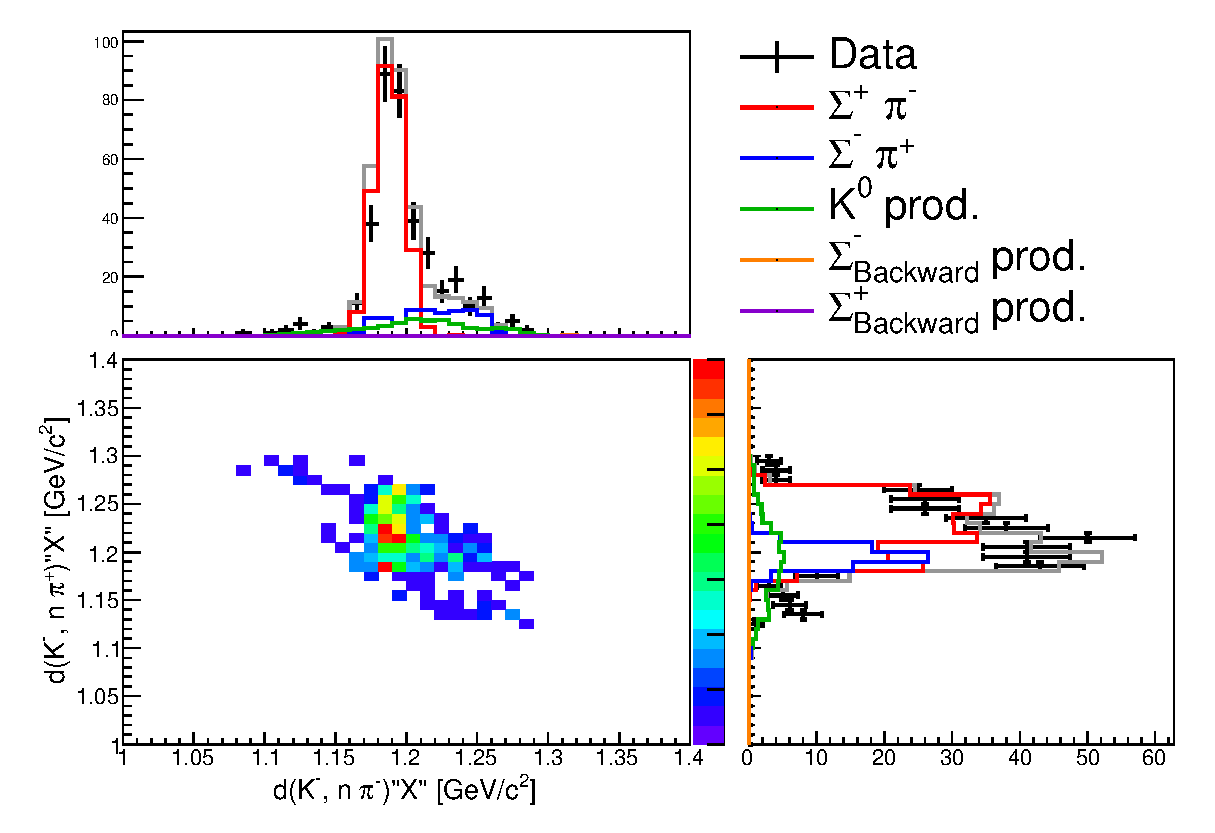
\includegraphics[width=2.2cm]{../pic/Run78/KN_ana_NC170_2sigma/KNpi_MM_12.eps}
    \end{minipage}
    \begin{minipage}{0.2\hsize}
      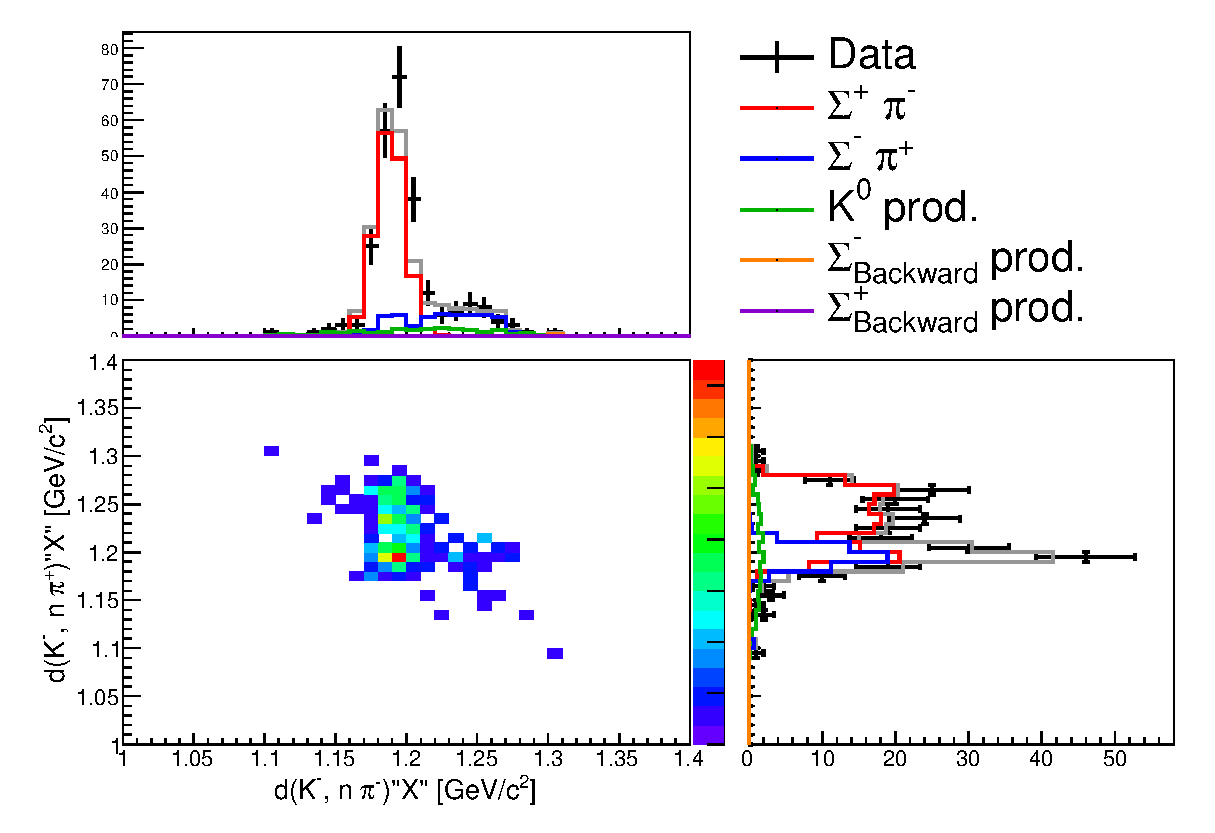
\includegraphics[width=2.2cm]{../pic/Run78/KN_ana_NC170_2sigma/KNpi_MM_13.eps}
    \end{minipage}
    \begin{minipage}{0.2\hsize}
      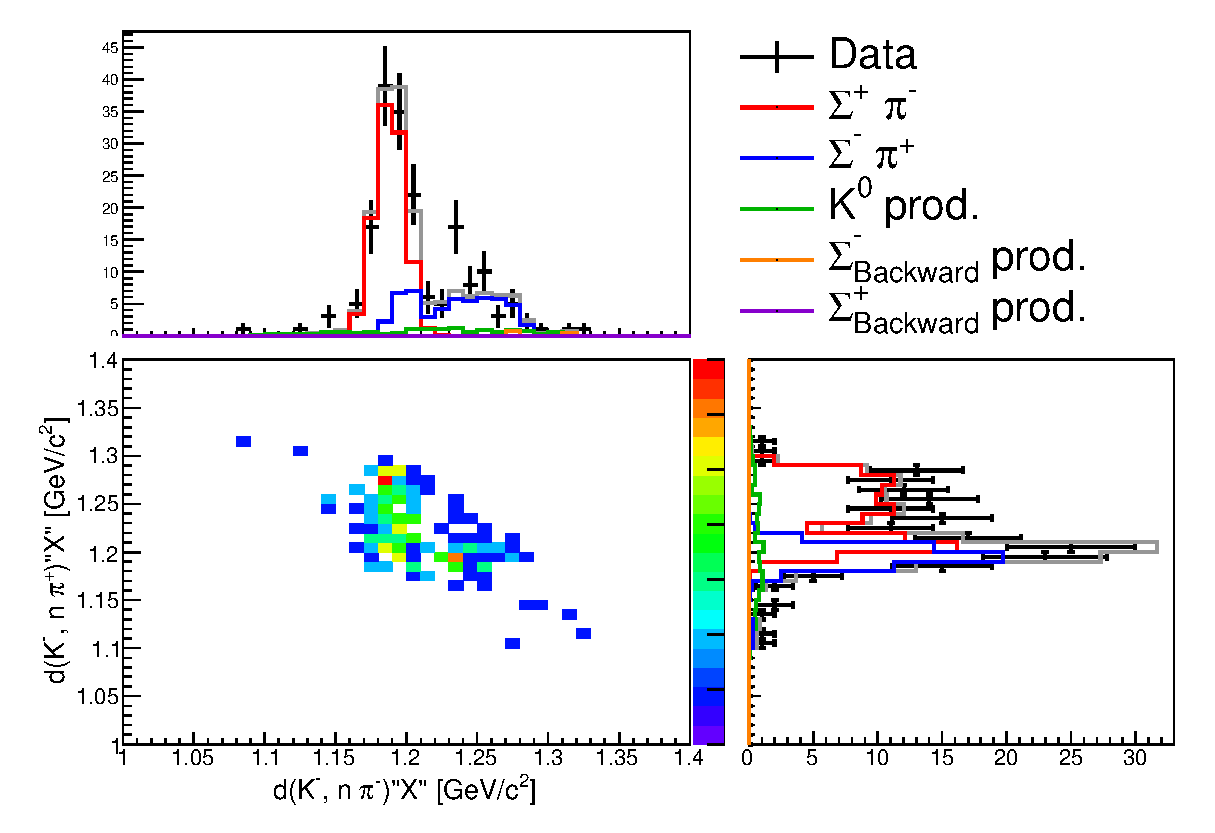
\includegraphics[width=2.2cm]{../pic/Run78/KN_ana_NC170_2sigma/KNpi_MM_14.eps}
    \end{minipage}
  \end{tabular}
  \begin{tabular}{ccccc}
    \begin{minipage}{0.2\hsize}
      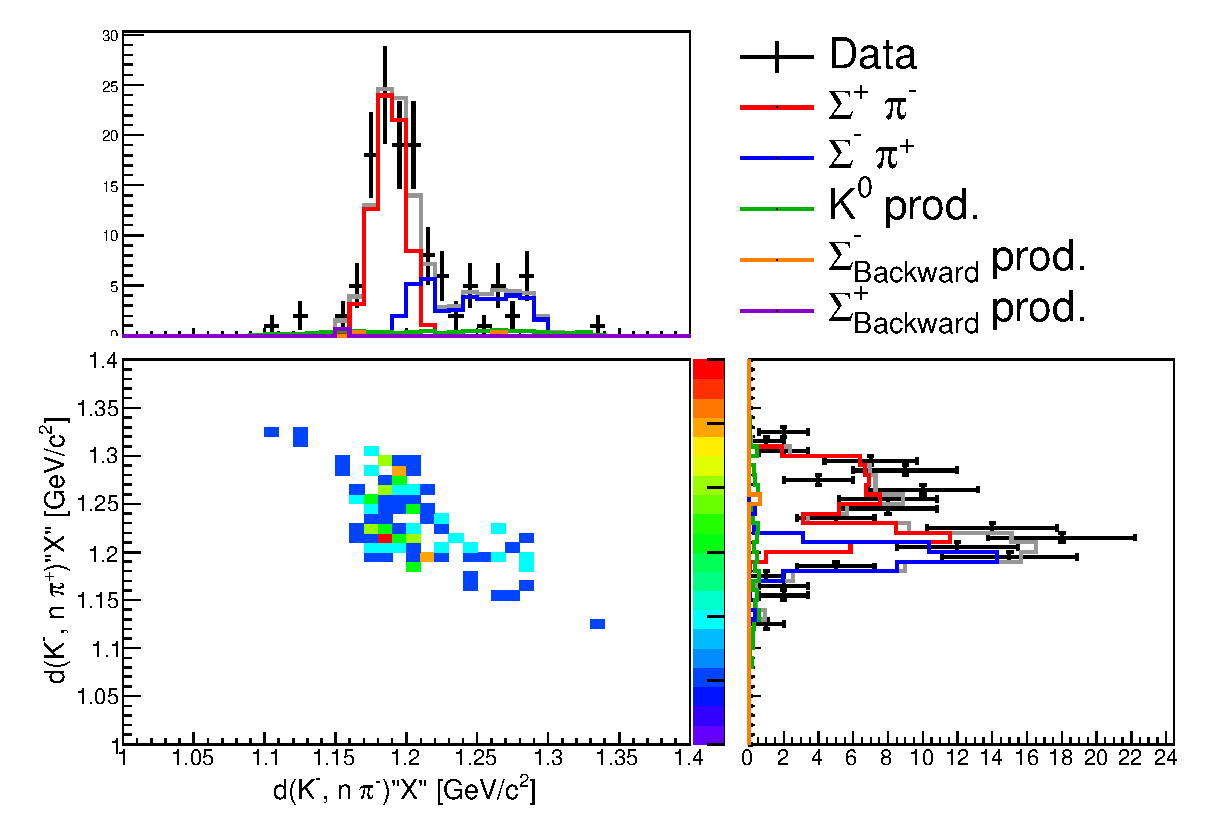
\includegraphics[width=2.2cm]{../pic/Run78/KN_ana_NC170_2sigma/KNpi_MM_15.eps}
    \end{minipage}
    \begin{minipage}{0.2\hsize}
      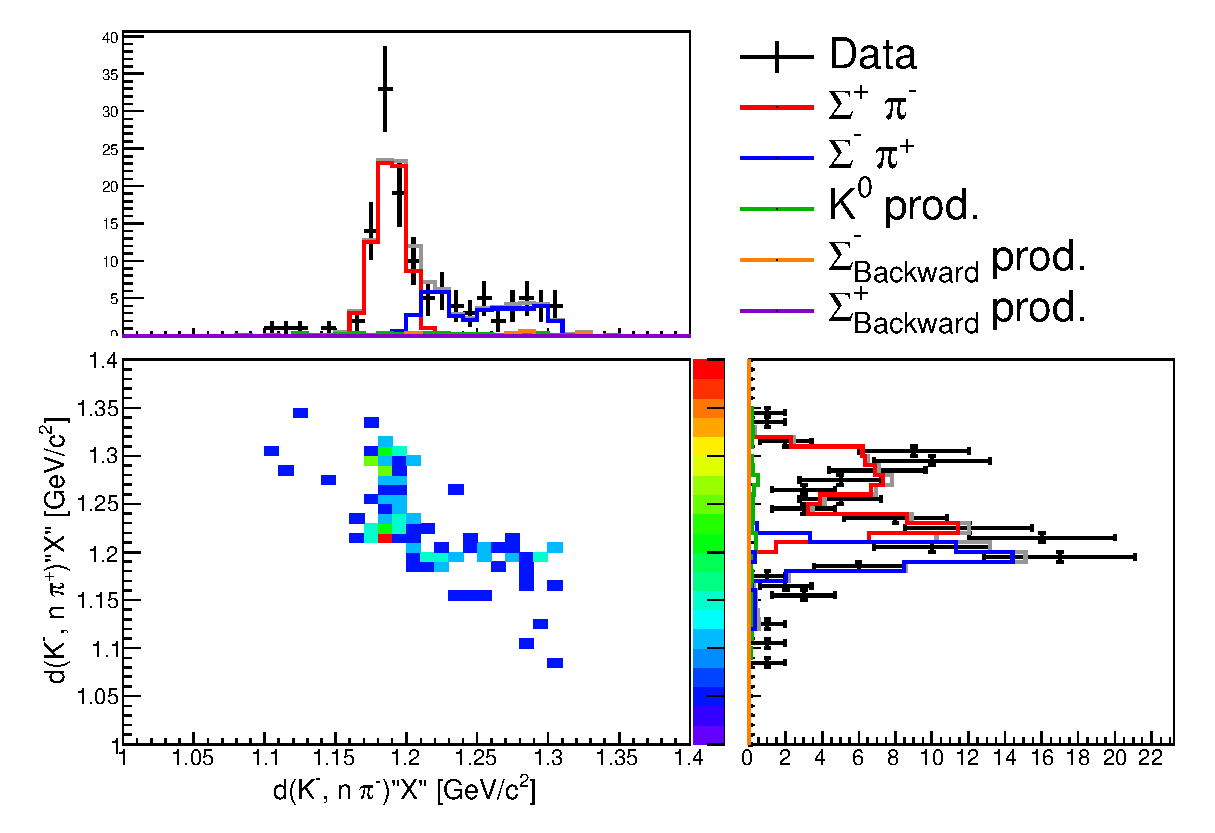
\includegraphics[width=2.2cm]{../pic/Run78/KN_ana_NC170_2sigma/KNpi_MM_16.eps}
    \end{minipage}
    \begin{minipage}{0.2\hsize}
      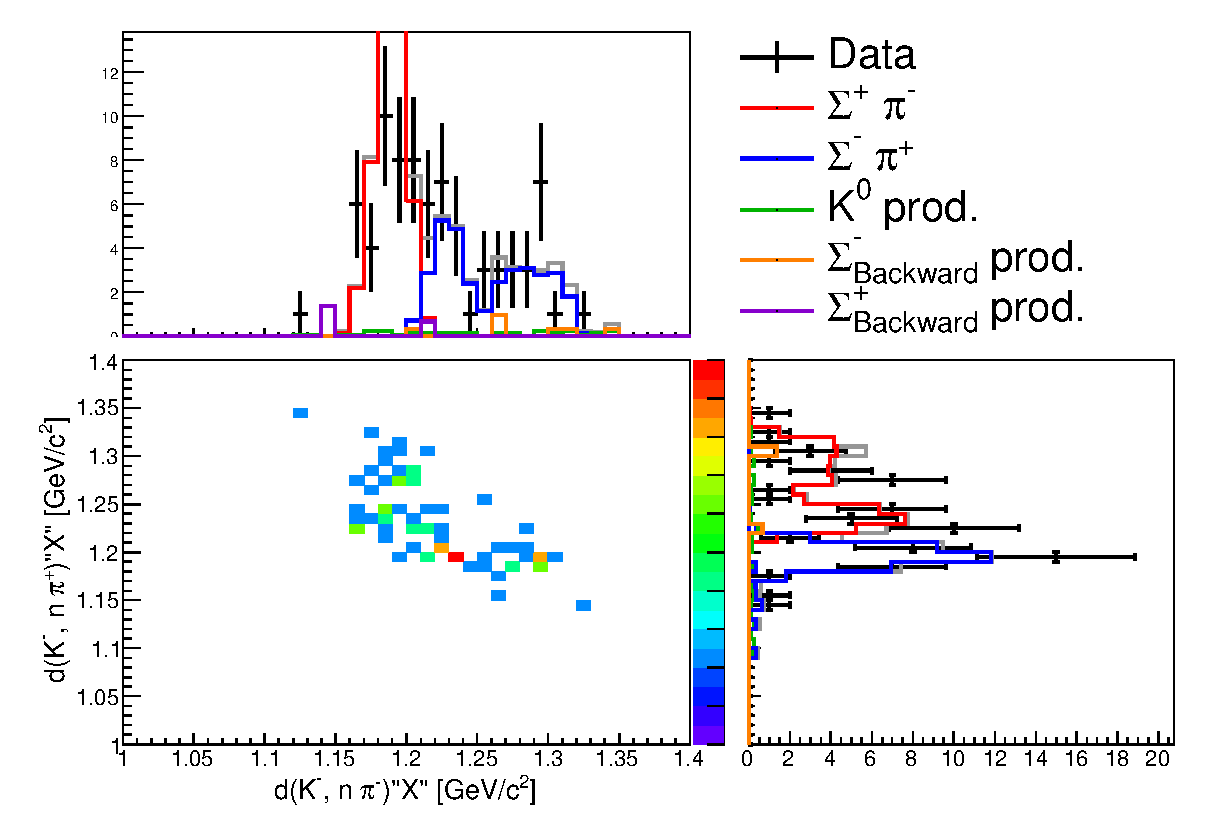
\includegraphics[width=2.2cm]{../pic/Run78/KN_ana_NC170_2sigma/KNpi_MM_17.eps}
    \end{minipage}
    \begin{minipage}{0.2\hsize}
      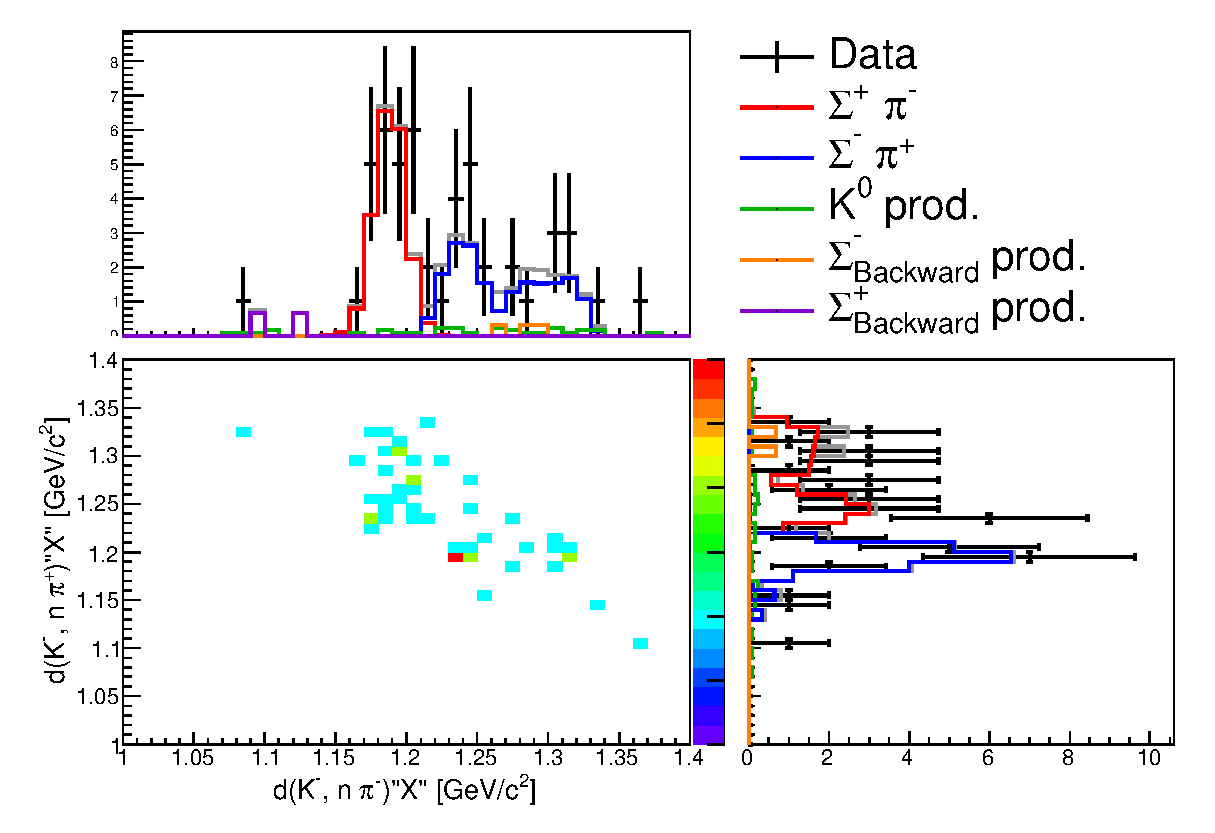
\includegraphics[width=2.2cm]{../pic/Run78/KN_ana_NC170_2sigma/KNpi_MM_18.eps}
    \end{minipage}
    \begin{minipage}{0.2\hsize}
      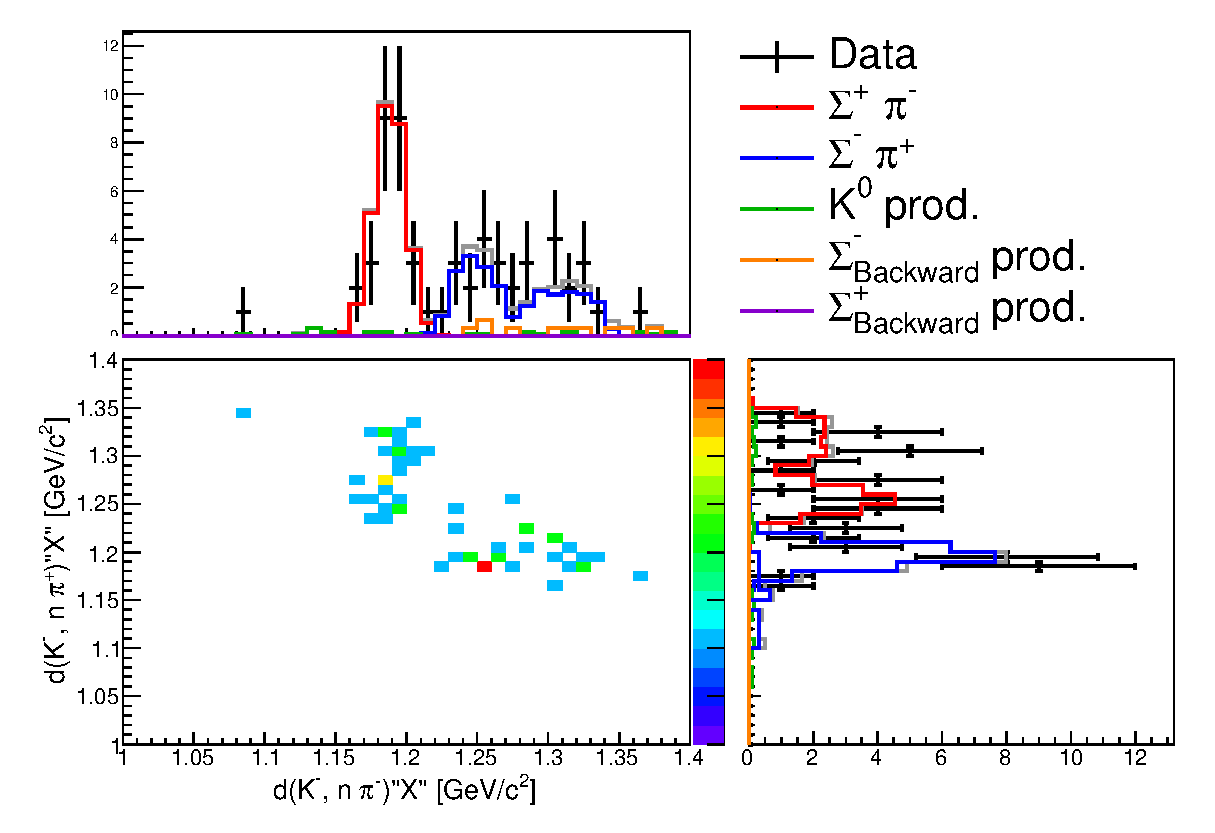
\includegraphics[width=2.2cm]{../pic/Run78/KN_ana_NC170_2sigma/KNpi_MM_19.eps}
    \end{minipage}
  \end{tabular}
  \begin{tabular}{ccccc}
    \begin{minipage}{0.2\hsize}
      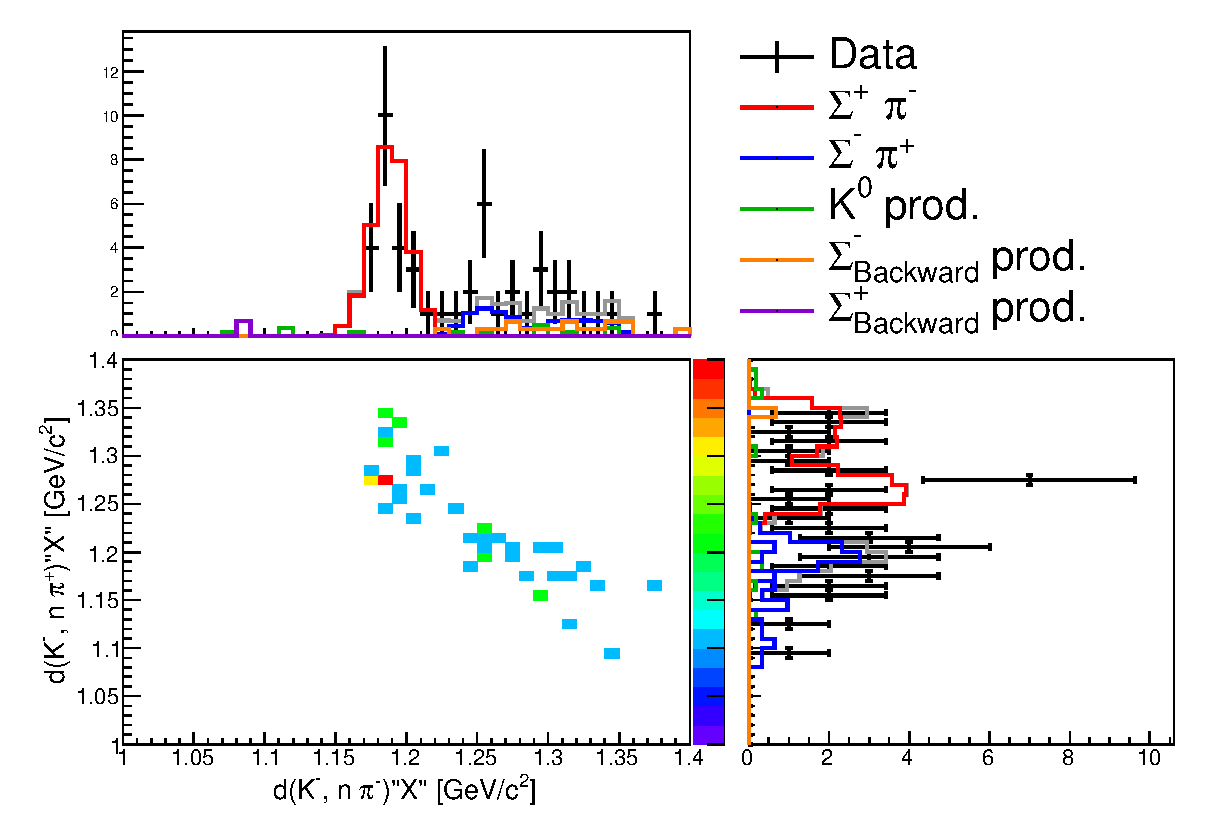
\includegraphics[width=2.2cm]{../pic/Run78/KN_ana_NC170_2sigma/KNpi_MM_20.eps}
    \end{minipage}
    \begin{minipage}{0.2\hsize}
      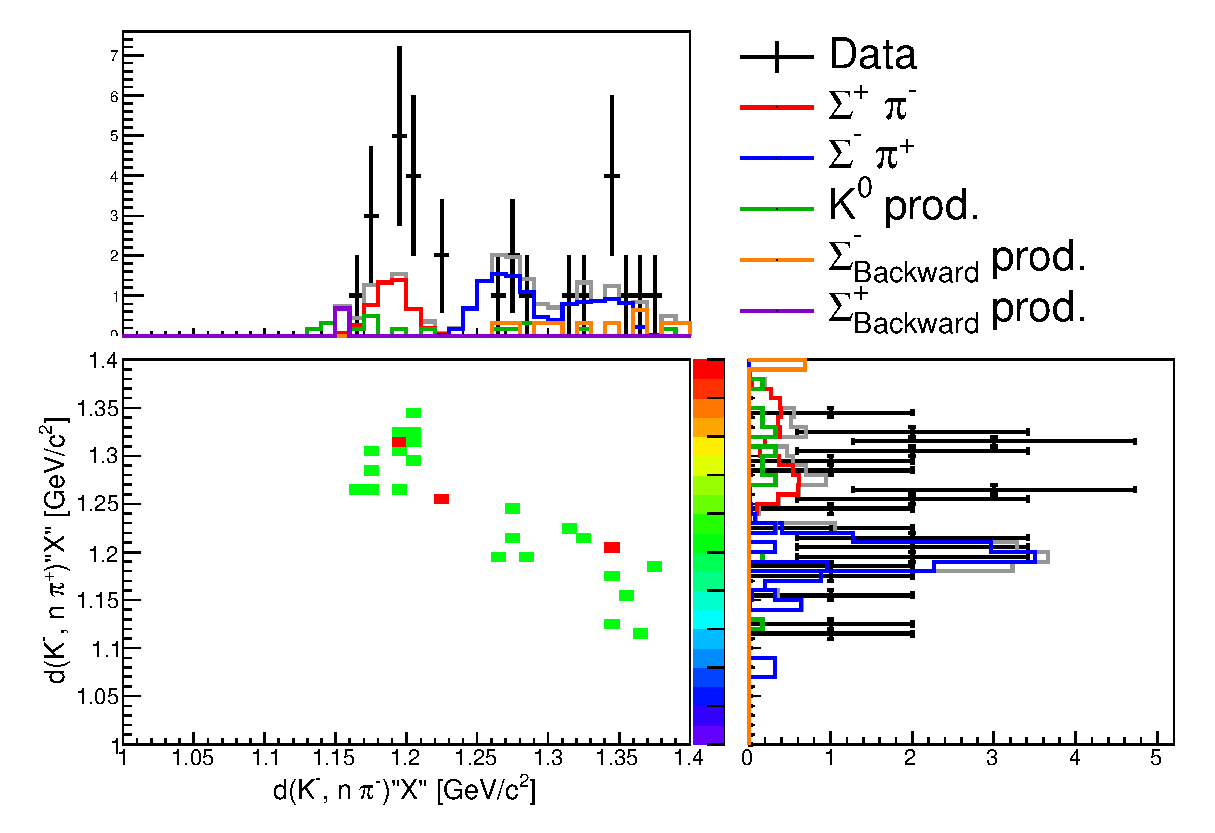
\includegraphics[width=2.2cm]{../pic/Run78/KN_ana_NC170_2sigma/KNpi_MM_21.eps}
    \end{minipage}
    \begin{minipage}{0.2\hsize}
      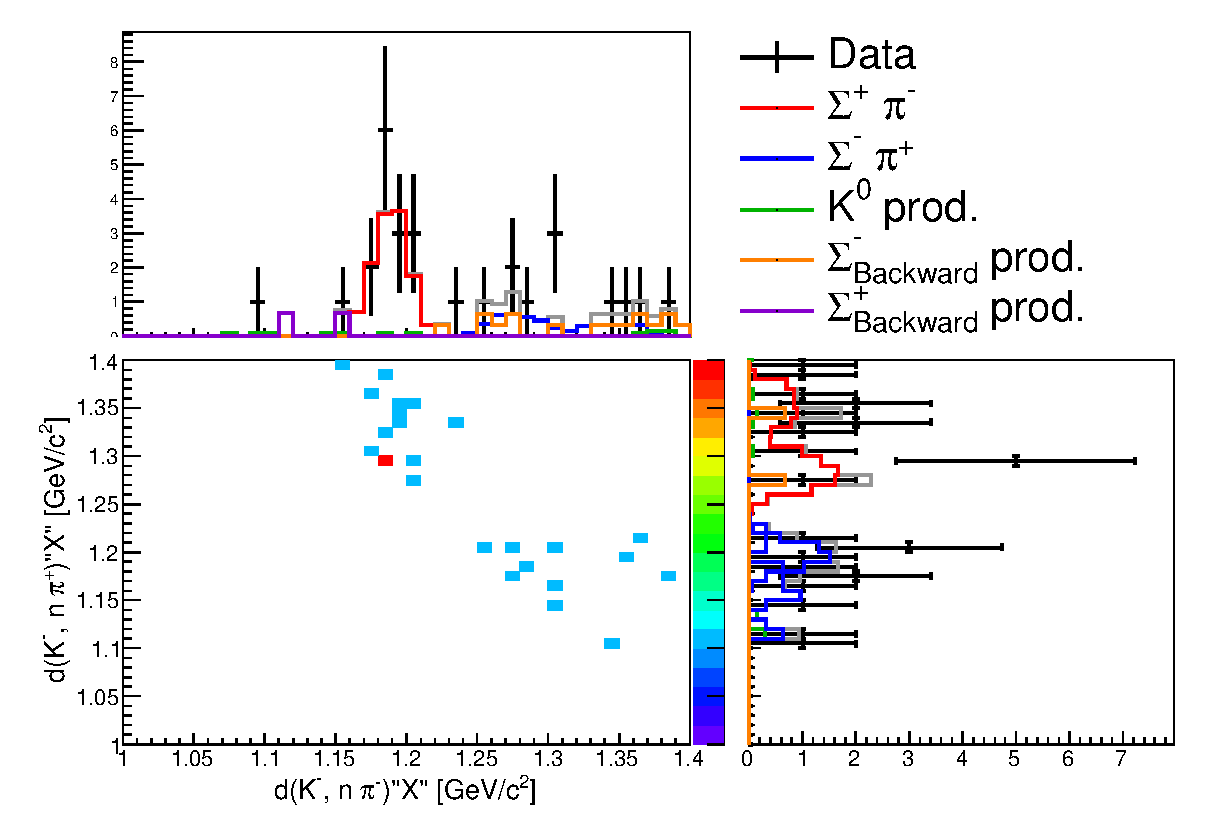
\includegraphics[width=2.2cm]{../pic/Run78/KN_ana_NC170_2sigma/KNpi_MM_22.eps}
    \end{minipage}
    \begin{minipage}{0.2\hsize}
      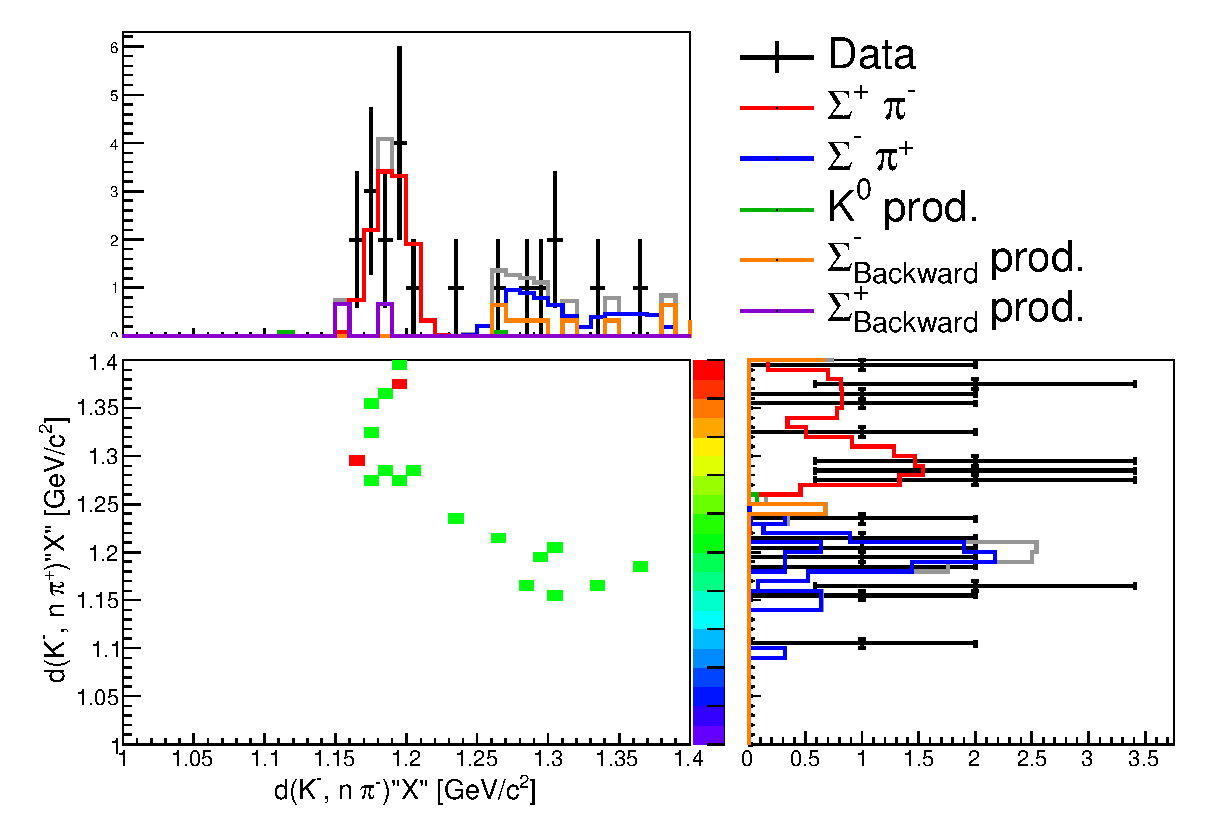
\includegraphics[width=2.2cm]{../pic/Run78/KN_ana_NC170_2sigma/KNpi_MM_23.eps}
    \end{minipage}
    \begin{minipage}{0.2\hsize}
      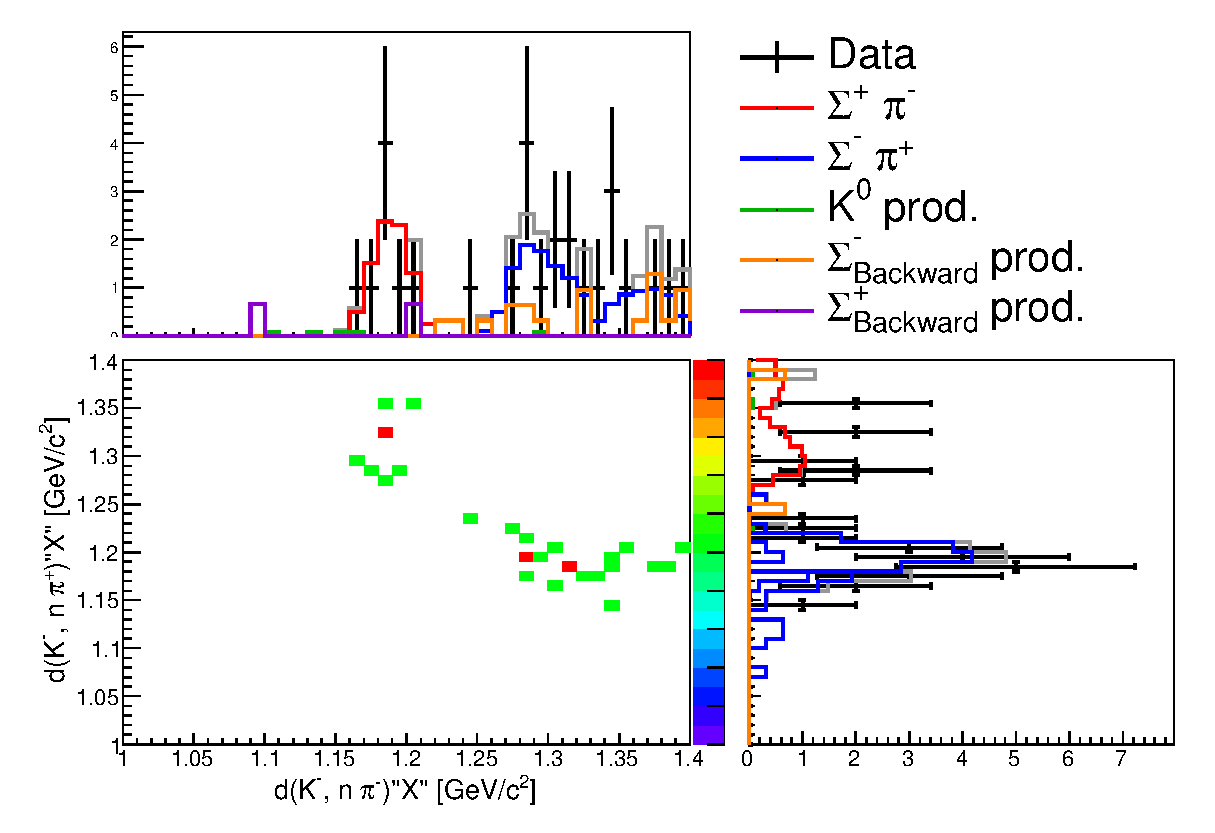
\includegraphics[width=2.2cm]{../pic/Run78/KN_ana_NC170_2sigma/KNpi_MM_24.eps}
    \end{minipage}
  \end{tabular}
  \label{fig:fit_KNpi_MM}
  \caption{
    These figures are presented separately for each bin of $d(K^-, n)$ for fitting to separate $\pi^- \Sigma^+$ and $\pi^+ \Sigma^-$ modes.
    The top left figure shows the lowest missing mass in the $1.35$-$1.36$GeV bin, with the next bin represented as one goes to the right.
    In other words, one row is shown for the 0.05GeV region.
  }
\end{figure}

\begin{figure}[htbp]
  \centering

  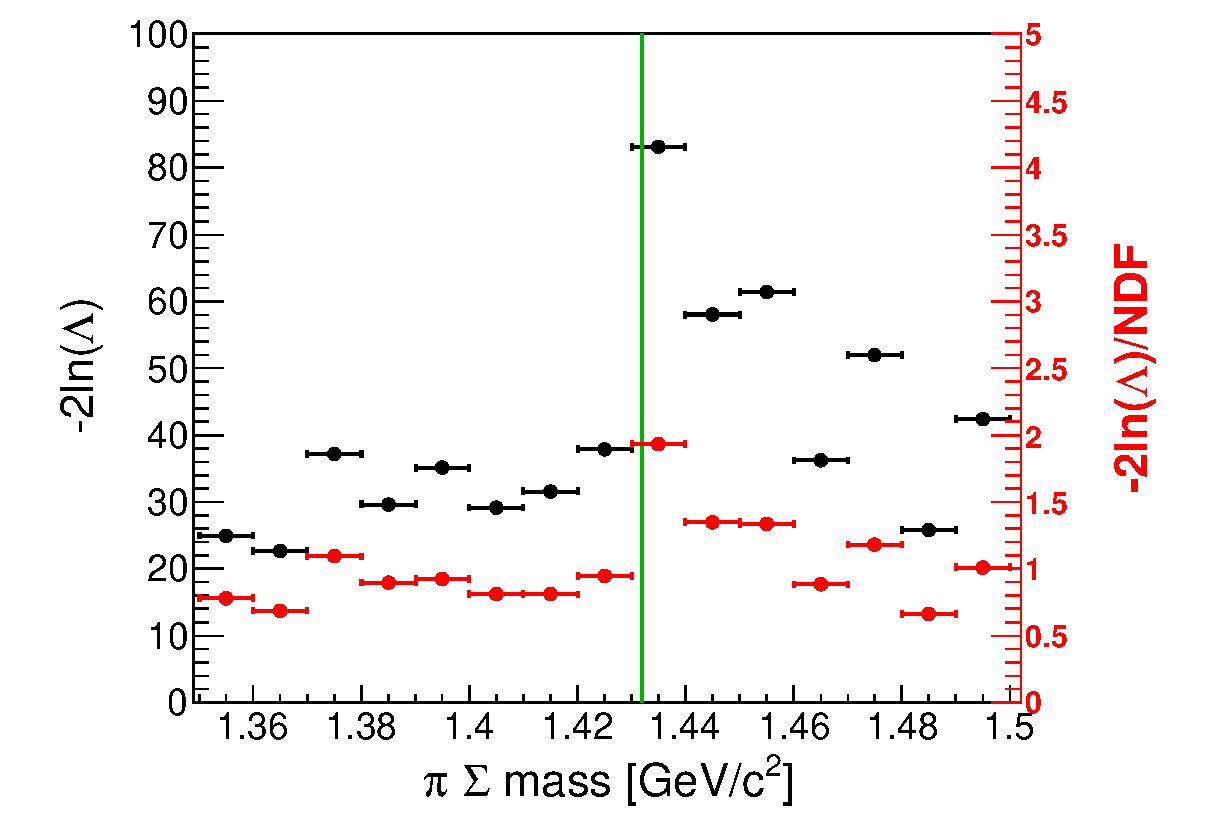
\includegraphics[width=8cm]{../pic/Dron/tempFit_KNpi_MM_Chi2.eps}
  \caption{
    This figure shows the template fitting $-2\log\Lambda$ and $-2\log\Lambda/NDF$ for the separation of $\pi^- \Sigma^+$ and $\pi^+ \Sigma^-$ modes in each $d(K^-, n)$ bin.
    Black and red indicate $-2\log\Lambda$ and $-2\log\Lambda/NDF$, respectively.
    The horizontal axis is represented for $d(K^-, n)$ bins.
  }
  \label{fig:tempFit_KNpi_Chi2}
\end{figure}


The fitting to separate the $\pi^-\Sigma^+$ and $\pi^+\Sigma^-$ modes is performed for events from $K^-- d \rightarrow n \pi^+ \pi- n$, excluding $K^0 $and $\Sigma^{\pm}_{forward}$ production.
However, the background leakage is estimated by scaling the distribution reconstructed in the MC simulation by the intensity estimated by the invariant mass fitting.
This fitting is performed each bin of the missing mass of $d(K^-, n)$, since the scattering amplitude of $\bar{K}N \rightarrow \pi \Sigma$ depends on the $\pi \Sigma$ invariant mass.
For this fitting we use the $d(K^-, n \pi^-)$ and $d(K^-, n \pi^+)$ missing masses as shown in Fig.\ref{fig:fit_KNpi_MM_all}.
This figure shows the sum of the $d(K^- , n)$ bins.
The bottom left figure shows a two-dimensional figure of the $d(K^-, n \pi^-)$ and $d(K^-, n \pi^+)$ missing masses on the horizontal and vertical axes, respectively.
The top and right figures show the projections of the respective axes.
The missing mass of $d(K^-, n \pi)$ makes a peak at $\Sigma$ for the correct combination for the missing $\Sigma$, but is widely distributed in the kinematic region for the opposite charge.
For example, for $d(K^-, n \pi^-)$, the $\pi^- \Sigma^+$ mode has a peak structure as shown by the red line,
whereas the $\pi^+ \Sigma^-$ mode has a widely distributed structure as shown by the blue line.

Fig.\ref{fig:fit_KNpi_MM} shows the results for the fitting of each bin of $d(K^-, n)$ separately.
Fig.\ref{fig:tempFit_KNpi_Chi2} shows the $-2\log\Lambda$ and $-2\log\Lambda/NDF$ of this fitting in each $d(K^-, n)$ bin in black and red, respectively.

Fitting to estimate background and to separate $\pi^- \Sigma^+$ and $\pi^+ \Sigma^-$ modes cannot be performed simultaneously as they use different event samples.
They are therefore repeated in the following steps.

First, the separation of $\pi^- \Sigma^+$ and $\pi^+ \Sigma^-$ modes is performed without considering the background.
The obtained distribution of backward $\pi^{\mp} \Sigma^{\pm}$ modes is used for fitting to estimate the background,
which is then fed back into the fitting of the separation of $\pi^- \Sigma^+$ and $\pi^+ \Sigma^-$ modes.
After five iterations of this procedure, fitting is performed considering 2-step and direct $\Lambda(1520)$ generation for $K^0$ generation, which is described in the Appendix.\ref{apendix:K0_event}.
Finally, fitting of the separation of the $\pi^- \Sigma^+$ and $\pi^+ \Sigma^-$ modes is performed to obtain the final $\pi \Sigma$ spectrum as shown in Fig.\ref{fig:piS_num}..

\begin{figure}[htbp]
  \centering
  
  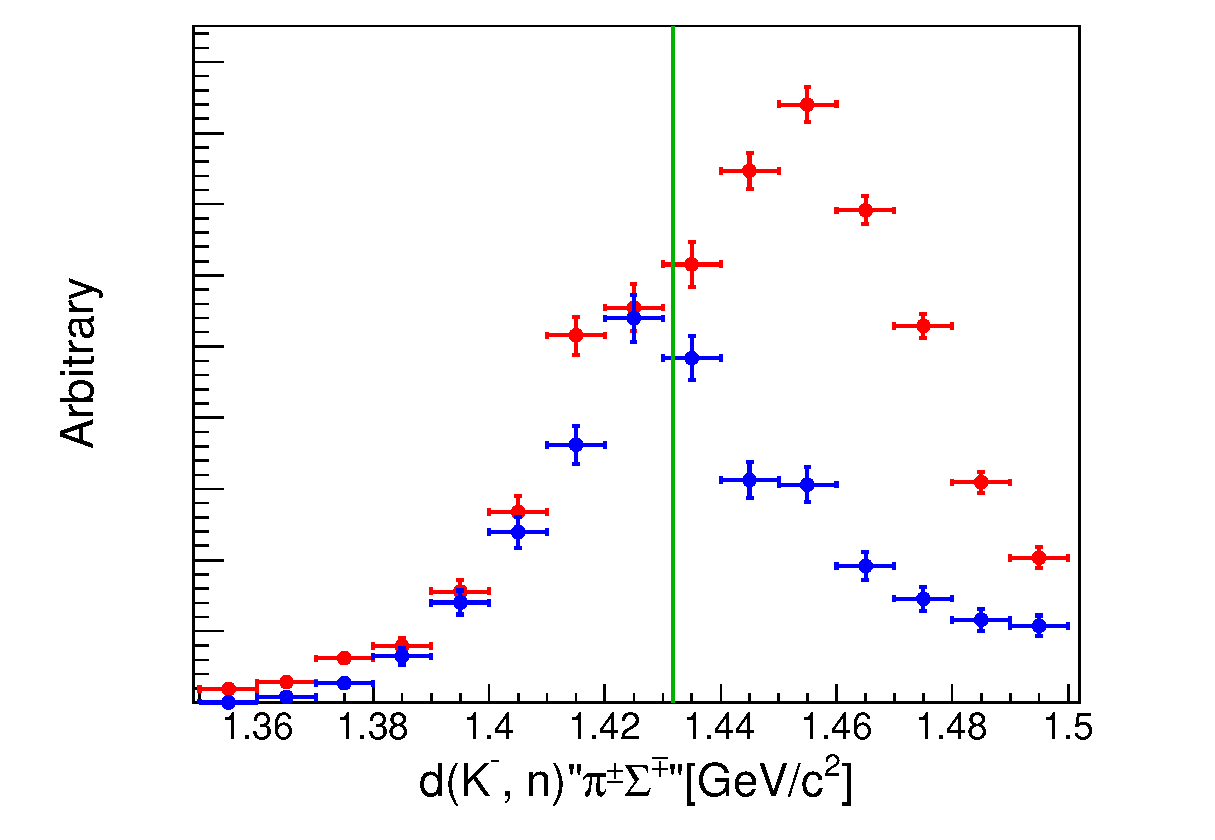
\includegraphics[width=8cm]{../pic/Dron/piS_num.eps}
  \caption{
    The $\pi^-\Sigma^+$ and $\pi^+\Sigma^-$ mode spectra obtained by template fitting are shown in arbitrary units.
    Red and blue lines indicate $\pi^-\Sigma^+$ and $\pi^+\Sigma^-$, respectively.
    The green vertical line is indicated the $\bar{K}N$ threshold.        
  }
  \label{fig:piS_num}
\end{figure}


